\documentclass[12pt, a4paper]{article}
% including images
\usepackage{graphicx}
\usepackage[margin=1in]{geometry}
\graphicspath{ {./figs/} }

% For links
%\usepackage{hyperref}
% For indent after new heading 
\usepackage{indentfirst}

% citations
\usepackage[backend=biber,style=ieee]{biblatex}
\addbibresource{report.bib}
% Chinese typesetting
\usepackage{xeCJK}
\setCJKmainfont{WenQuanYi Micro Hei Mono}
\usepackage{setspace}

\begin{document}
\newcommand{\largeTitle}[1]{\fontsize{40}{50} #1}

%---------- TITLE PAGE ---------- 
% TODO: Fix the fonts to make it more professional
\begin{titlepage}
		\begin{center}
			\largeTitle \textbf{國立交通大學} \\[0.25cm]
			\largeTitle \textbf{資訊工程學系} \\[0.25cm]

			\LARGE{Lo mismo en chino} \\[0.5cm]

			\LARGE{Intelligent Image Processing for Aerial 2-D Image Stitching}
		\end{center}

		\vspace{\fill}
		% bottom half of title page
		% TODO: This looks quite weird
		\begin{tabular}{c l}
			{\makebox[8em][s]{\LARGE 大學生}} & \LARGE Andr\'es Ponce 彭思安 \\[0.5cm]
			{\makebox[8em][s]{\LARGE 指導教授}} & \LARGE Maria Yuang 楊啟瑞 \\[0.5cm]
		\end{tabular}

		\vspace{3cm}
		% TITLE PAGE FOOTER
		\begin{center}
			{\LARGE 中華民國 109 年 12 月 27日}
		\end{center}
\end{titlepage}

% ---------- ABSTRACT ----------
\section{Abstract}
\label{sec:Abstract}
Intelligent Image Processing is one of the subtask of 5G-DIVE Autonomous Drone Scout (ADS) verticals. It 
aims  to  intelligently  compute  drone  video  stream  in  the  edge  to  detect  persons  in  need  of  help,  and  to 
provide stitched image of a disaster impacted area. 5G-DIVE project is a collaborative project between the 
EU  and  Taiwan  to  prove  the  technical  merits  and  business  value  preposition  of  5G  technologies  in  ADS 
vertical pilot. In this research project, we worked on an improved Aerial 2D-ST solution that leverages the 
5G-DIVE platform specifically the IESS to improve 2D-ST. In particular, AI techniques is used as a solution to 
improve on the existing 2D-ST solution to produce high-quality stitched image but without sacrificing for 
computation time.

\section{Introduction}
\label{sec:Introduction}
A panorama in visual art depicts a continuous scene or landscape~\cite{Panorama}. 
The concept of panoramas in photoraphy has existed for centuries. 
In the middle of the 19$^{th}$ century, landscapes were created by placing daguerrotypes side by side
side by side~\cite{OhioStitching}. Panorama images have been popularized in the last
years due to their widespread inclusion in smartphones and digital cameras; for example,
the iPhone5 introduced panoramic images in 2012~\cite{iPhoneStitch}. As processing
power has grown, new and increasingly smart solutions have allowed better quality
images to be stitched for pleasing results.

In digital photography, a panoramic image refers to a large composite image made of 
smaller images with overlapping areas. 
Computer software will look for the optimal way to combine the overlapping areas of the 
images such that the output panorama exhibits little or no visual artifacts. 
Image stitching has multiple uses other than recreative or artistic, producing
a map of an area from overhead drone image~\cite{OpenDroneMapTheMissingGuide}, or 
for medical imaging applications.


\begin{figure}[b]
		\label{fig:PanoExample}
		\centering
		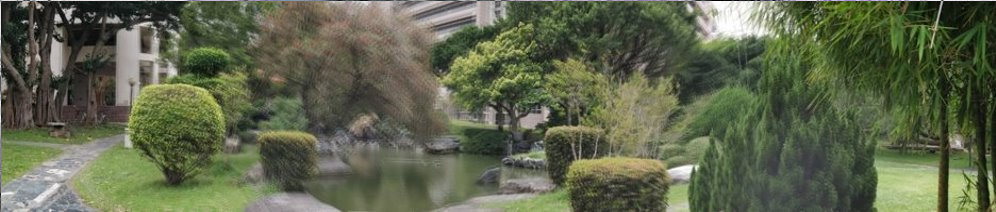
\includegraphics[scale=0.4]{pano.png}
		\caption{Example of stitched image. However, some visual artifacts might 
		still remain in the final image.}	
\end{figure}

\section{Problem Description}
\label{sec:ProblemDescription}
The problem of focus here involves designing and implementing an image stitching 
pipeline that is robust yet has low latency. The input will be a series of images
taken by a drone, and the output will be a single high-resolution panorama image.

An envisioned usage scenario would involve drones capturing video footage 
over an area impacted by some disaster. This footage is then to be transmitted 
to a server for stitching. Using the stitched images, a clearer representation of the 
impacted area should be visible, in case detecting persons in need of help or
producing a clearer picture of the area was necessary. 

\section{Existing Literature}
\label{sec:Literature}

The original paper on image stitching~\cite{brown2007automatic} introduces a 
pipeline with several steps: feature matching, image matching, bundle adjustment,
panorama straightening and blending. Many individual projects implement this 
pipeline and even some professional projects. OpenCV's image stitching module
utilizes this pipeline to stitch multiple images together.

Next is a brief description of the pipeline according to the original paper:
\begin{enumerate}
		\item \textbf{Image Matching}: In this stage we find the regions of 
				interest in each image of the sequence. A region of interest,
				commonly called a feature, could represent an area of the image
				with large variations in pixel intensities. Once a feature is 
				found, relevant information about it is stored in a k-d tree.


\end{enumerate}
\section{Resolution Method}
\label{sec:ResolutionMethod}

\section{System Design and Implementation}
\label{sec:DesignAndImplementation}

\section{Result Analysis}
\label{sec:Results}

\section{Conclusions and Contributions}
\label{sec:Conclusion}

\vspace{\fill}

\printbibliography
\end{document}
